\documentclass{sig-alternate}

\usepackage{graphicx}
\usepackage{xcolor}
\newcommand\todo[1]{\textcolor{red}{#1}}



\begin{document}
\conferenceinfo{SIGMOD}{Snowbird, Utah USA}
\title{COMB - Do We Really Need Full Indexing?}
\numberofauthors{4}
%\author{
%\alignauthor
%Felix Halim\\
%       \affaddr{Google Inc}\\
%       \email{felixhalim@google.com}
%\alignauthor
%Stratos Idreos\\
%       \affaddr{Centrum Wiskunde Informatica}\\
%       \email{S.Idreos@cwi.nl}
%\alignauthor Panagiotis Karras\\
%       \affaddr{Rutgers}\\
%       \email{karras@business.rutgers.edu}
%\and
%\alignauthor Roland Yap\\
%       \affaddr{National University of Singapore}\\
%       \email{ryap@comp.nus.edu.sg}
%}

\date{17 Sept 2013}

\maketitle
\begin{abstract}
\todo{Explain data deluge problem and how adaptive indexing addressed the problem.
However, it fails (as we show) under heavy updates and/or large number of queries. }

\todo{This paper proposes COMB, a much more efficient cracking data structure.
COMB can be augmented to "crack" any other in-memory data structure.
We show how to use COMB to {\em crack} BTree and ART to achieve 
very low initialization cost,
and still match or better under long queries and under heavy updates.
COMB effectively eliminates the need to use full indexing.
}

\end{abstract}

%\category{H.4}{Information Systems Applications}{Miscellaneous}
%\category{D.2.8}{Software Engineering}{Metrics}[complexity measures, performance measures]

%\terms{Theory}
%\keywords{ACM proceedings, \LaTeX, text tagging}

\section{Introduction}

\todo{Explain data deluge challenge, importance of physical design,
dynamic workload, adaptive indexing.}

\todo{Motivate the need for improvement \cite{felix14uncracked}.
This paper is the answer to all the shortcomings of cracking.}

\todo{Explain that Cracking is a concept of incrementally build index
as a side effect of query processing.
This concept is general and can be applied anywhere.
Database Cracking is one implemenation of that concept.}

\todo{The problem is Database Cracking implementation uses plain array
and AVL tree for the cracker indexes.
As the result, the benefit of DB Cracking is only seen for small number of 
(read only) queries \cite{felix14uncracked}
(i.e., less than a few thousands before it loses to other data structures).
Moreover, as we shall see, under heavy updates, DB Cracking is impractical.}

\todo{comb no worse than sort in amortized cost and do far better than sort in the meantime}

\todo{In this paper, we propose COMB, a new data structure that allows
efficient transformation from unindexed to full index with little or negative overhead.
The innovation in the design of COMB, is that it breaks a single column into multiple
disjoint pieces and each piece is indexed, accessed and updated independently,
while data flows from piece to piece in an adaptive way {\em as necessary}
when the index needs to be refined.}

\todo{New in-memory data structure can adopt the COMB data structure
and enjoy the low initialization cost without much overhead
(in fact, we see an overall speedup when integrated with COMB).
We show how to use COMB to {\em crack} BTree and ART (the current state
of the art in-memory index).}

\begin{figure}
\centering
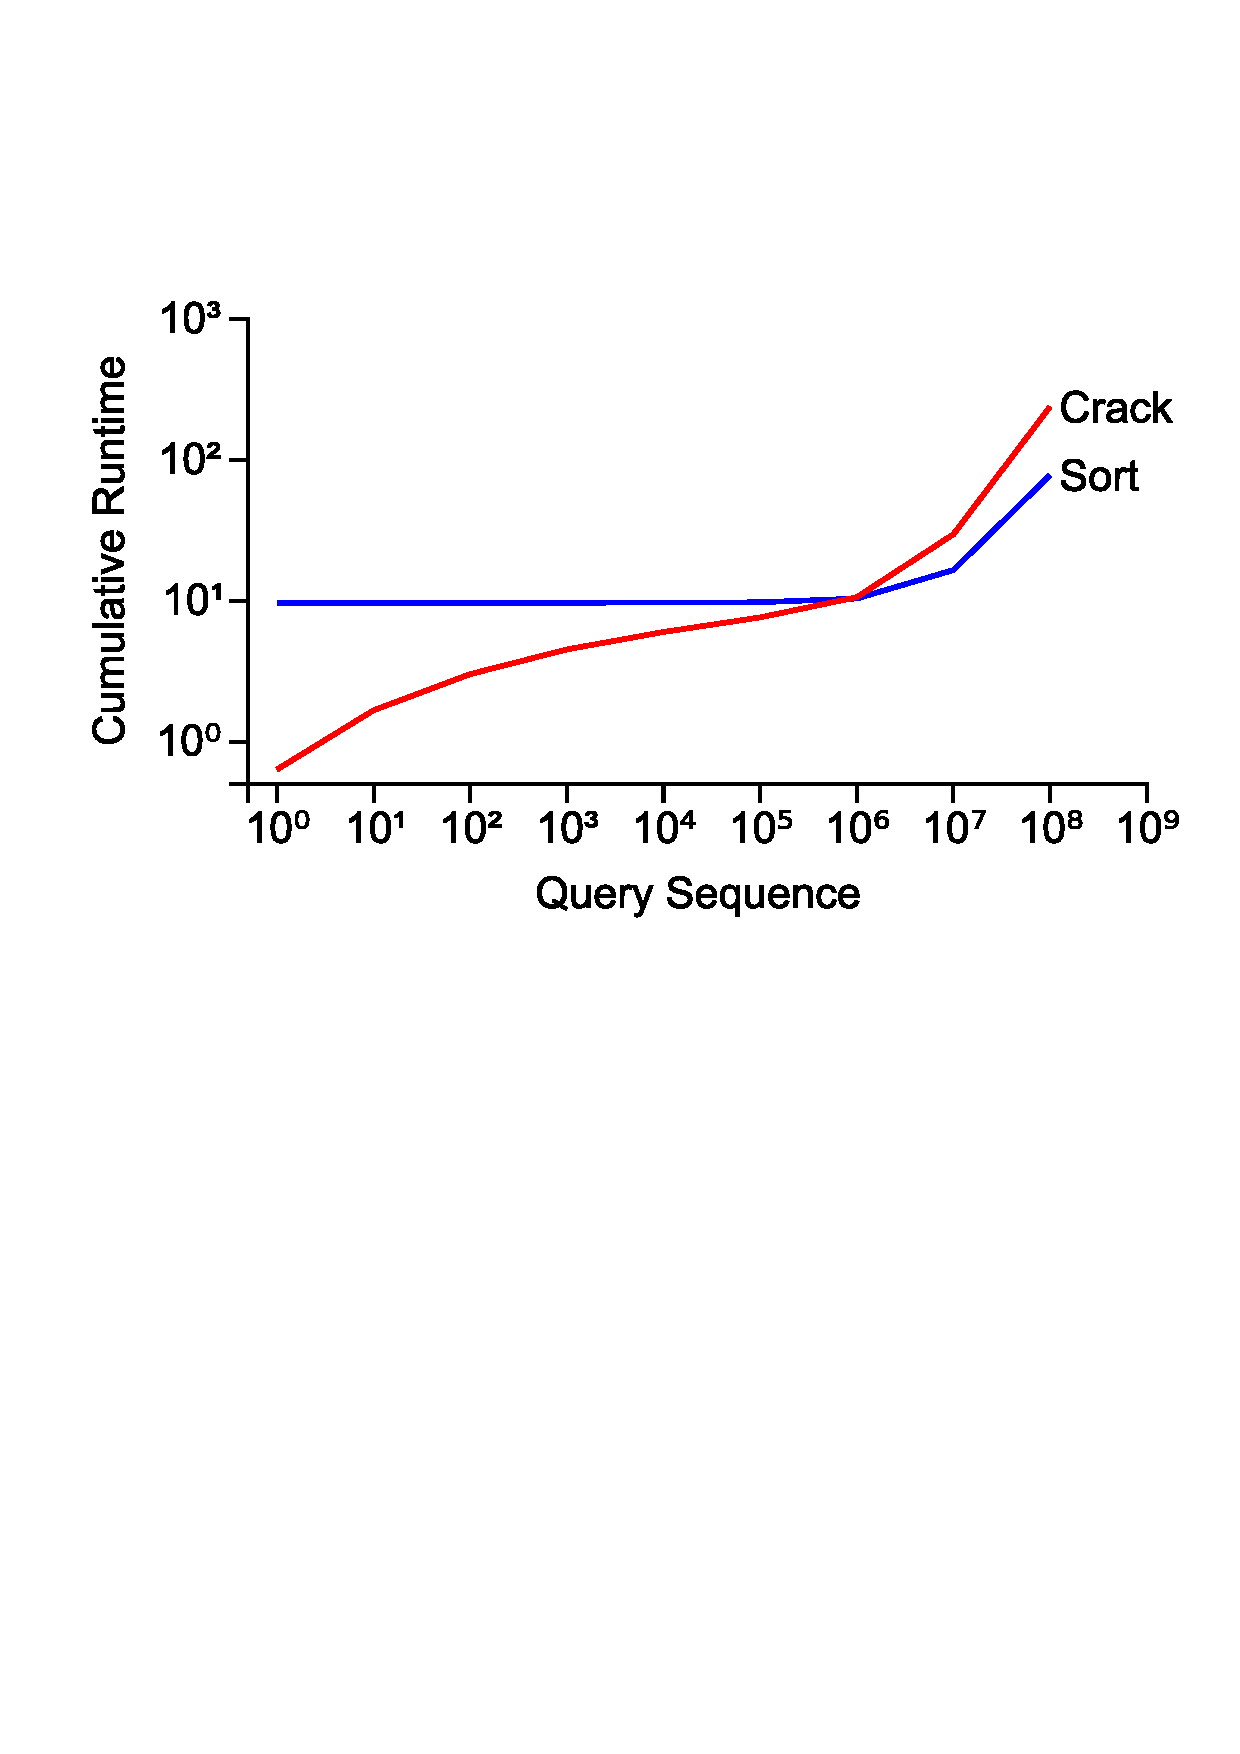
\includegraphics[width=0.5\textwidth]{crack_vs_sort.pdf}
\caption{A sample black and white graphic (.eps format)
that has been resized with the \texttt{epsfig} command.}
\end{figure}

\todo{Paper organization...}

\section{Related Work}

\todo{In \cite{felix14uncracked}, the evaluation is only for read queries.
This paper evaluates the update queries performance.}

In this paper we look at Cracking as a more general data structure.

- CTree evolves from database cracking, in the quest of finding efficient data structure to support incremental indexing as side effects of query processing.
- CTree is immune to selectivity.
- Compare with ART.
- Index Space consumption.
- CrackInTwo/Tree are obsolete, enter Fusion.
- Root array can be implemented using sorted data structure like ART, BTree, plain sorted array.

- Indexing signatures?
- BufferedSwapping?
- Coarse Granular Indexing better than scrack? it pre-crack into X coarse partitions. further cracks are inside each partitions.
this destroys the lightweightness of database cracking, it only shifts the work to earlier part of the queries.
if you race, the coarse granular indexing will lose.

- ART 3.6x faster on domain size? It should be slower on diverse size.

- Data Access dominates index lookup -> depends whether the query is a select all? or count queries.

Graph:
Index Lookup
Data Shuffle
Index Update
Data Access

- How quick is the convergence of CTree? it is at most log(N) indexes per compared to 2 in cracking.

- I think the latency comparison is unfair since sort assumes idle time, while cracking is not. if given idle time, cracking won't be worse than sort.
At 1000 th query, sort hasn't even finished indexing while cracking already answer 1000th query.

Race For Answering Queries
X axis: timeline.
Y axis: number of queries answered.

Plot number of swaps.

Fusion experiments.

Payload (for covered cracking).


Here is the SLA of database cracking: It will never worse than full index.

CTree: the best indexing strategy when no workload knowledge and idle time.
We demonstrate this on any number of queries and any workload we can think of.

We try to solve 2 problems:
- under heavy 

Cracking has disadvantages on heavy updates while btree / art does not.
It requires auxiliary data structure like AVL tree which is sub-optimal.

\section{Experiments}

\todo{explain the SLA as cumulative not individual}

\subsection{Fusion}
\subsection{Read Queries}
\subsection{Update Queries}
\subsection{Convergence}
\subsection{Robustness}
\subsection{Memory Consumption}
\subsection{Update Queries}


\begin{table}
\centering
\caption{CTree on NOUP}
\begin{tabular}{|c|c|l|} \hline
\textbf{Algorithms} & \textbf{Insert Time} & \textbf{Query Time}\\ \hline
CTree & 0.1 & 1 \\ \hline
BTree & 10 & 2 \\ \hline
RBTree & 20 & 4 \\ \hline
ART & 10 & 7 \\ \hline
\hline\end{tabular}
\end{table}



\begin{figure}
\centering
\epsfig{file=fly.eps}
\caption{A sample black and white graphic (.eps format).}
\end{figure}



\begin{figure*}
\centering
\epsfig{file=flies.eps}
\caption{A sample black and white graphic (.eps format)
that needs to span two columns of text.}
\end{figure*}

\begin{proof}
Suppose on the contrary there exists a real number $L$ such that
\begin{displaymath}
\lim_{x\rightarrow\infty} \frac{f(x)}{g(x)} = L.
\end{displaymath}
Then
\begin{displaymath}
l=\lim_{x\rightarrow c} f(x)
= \lim_{x\rightarrow c}
\left[ g{x} \cdot \frac{f(x)}{g(x)} \right ]
= \lim_{x\rightarrow c} g(x) \cdot \lim_{x\rightarrow c}
\frac{f(x)}{g(x)} = 0\cdot L = 0,
\end{displaymath}
which contradicts our assumption that $l\neq 0$.
\end{proof}

\section{Conclusions}


%!TEX encoding = UTF-8 Unicode\section{Acknowledgments}
%This section is optional; it is a location for you
%to acknowledge grants, funding, editing assistance and
%what have you.  In the present case, for example, the
%authors would like to thank Gerald Murray of ACM for
%his help in codifying this \textit{Author's Guide}
%and the \textbf{.cls} and \textbf{.tex} files that it describes.

\bibliographystyle{abbrv}
\bibliography{sigproc}  % sigproc.bib is the name of the Bibliography in this case

\end{document}
